\subsection{Übersetzung \hfill ME}
\begin{minipage}{0.68\linewidth}
    \begin{center}
        \begin{footnotesize}
        \begin{empheq}[box=\fbox]{align*}
            &i = \frac{\omega_{1(\text{an})}}{\omega_{2(\text{ab})}} = \frac{n_{1(\text{an})}}{n_{2(\text{ab})}} = \frac{d_{tk{2(\text{ab})}}}{d_{tk{1(\text{an})}}}
            \\ & = \frac{M_{2(\text{ab})}}{\eta M_{1(\text{an})}} = \frac{z_{2(\text{ab})}}{z_{1(\text{an})}}
        \end{empheq}
        \vspace{-2mm}
        \mathbox{
            i_{\text{ges}} = i_{1,2} \cdot i_{3,4} \cdot i_{5,6} = \frac{z_2 \cdot z_4 \cdot z_6}{z_1 \cdot z_3 \cdot z_5}
        }
        \vspace{-3mm}
        \mathbox{
            d_{tk} = \frac{U_{tk}}{\pi} = z_x \cdot \frac{p}{\pi} = z_x \cdot m
        }
        \vspace{-3mm}
        \mathbox{
            d_{a} = d_{tk} + 2 \cdot m
        }
        \vspace{-3mm}
        \mathbox{
            Z_g = \frac{2}{\sin(\alpha)^2}        
            }
            \vspace{-3mm}
            \mathbox{
                N_2 = \frac{r_1}{r_2} \cdot n_1 \; M_2 = \frac{r_2}{r_1} \cdot M_1
            }
        \end{footnotesize}
    \end{center}
\end{minipage}
\begin{minipage}{0.31\linewidth}
    \begin{center}
        \begin{scriptsize}
        \begin{align*}
            &\text{$i$ = Übersetzung};
            \\ &\text{$i < 1$: Abtr. schneller;}
            \\ &\text{$i > 1$: Abtr. langsamer;}
            \\ &\text{$\omega_x$ = Winkelgeschw.};
            \\&\text{$n_x$ = Drehzahl};
            \\&\text{$d_{tk}$ = Teilkreisdurchm.;}
            \\&\text{$M_x$ = Drehmoment;}
            \\&\text{$\eta$ = Wirkungsgrad;}
            \\&\text{$z_x$ = Zähnezahl};
            \\ &\text{$U_{tk}$ = Teilkreisumfang};
            \\ &\text{$p$ = Teilung};
            \\ &\text{$m$ = Modul \textcolor{Red}{= const.}};
            \\ &\text{$d_a$ = Aussendurchm.};
            \\ &P_{ab/an} = \text{Leistung};
            \\ &Z_g = \text{Grenzzähnezahl}
        \end{align*}
        \end{scriptsize}
    \end{center}
\end{minipage}

\vspace{2mm}

\center{\footnotesize{Weitere Beziehungen:}}
\begin{footnotesize}
    \vspace{-1mm}\mathbox{
    m = \frac{p}{\pi} \; \mid \; \omega_x = 2\pi n_x \; \mid \; \eta = \frac{P_{ab}}{P_{an}} = \frac{M_2n_2}{M_1n_1} = \frac{M_2}{M_1i} < 1
}
\end{footnotesize}
\begin{minipage}{0.58\linewidth}
    \begin{center}
        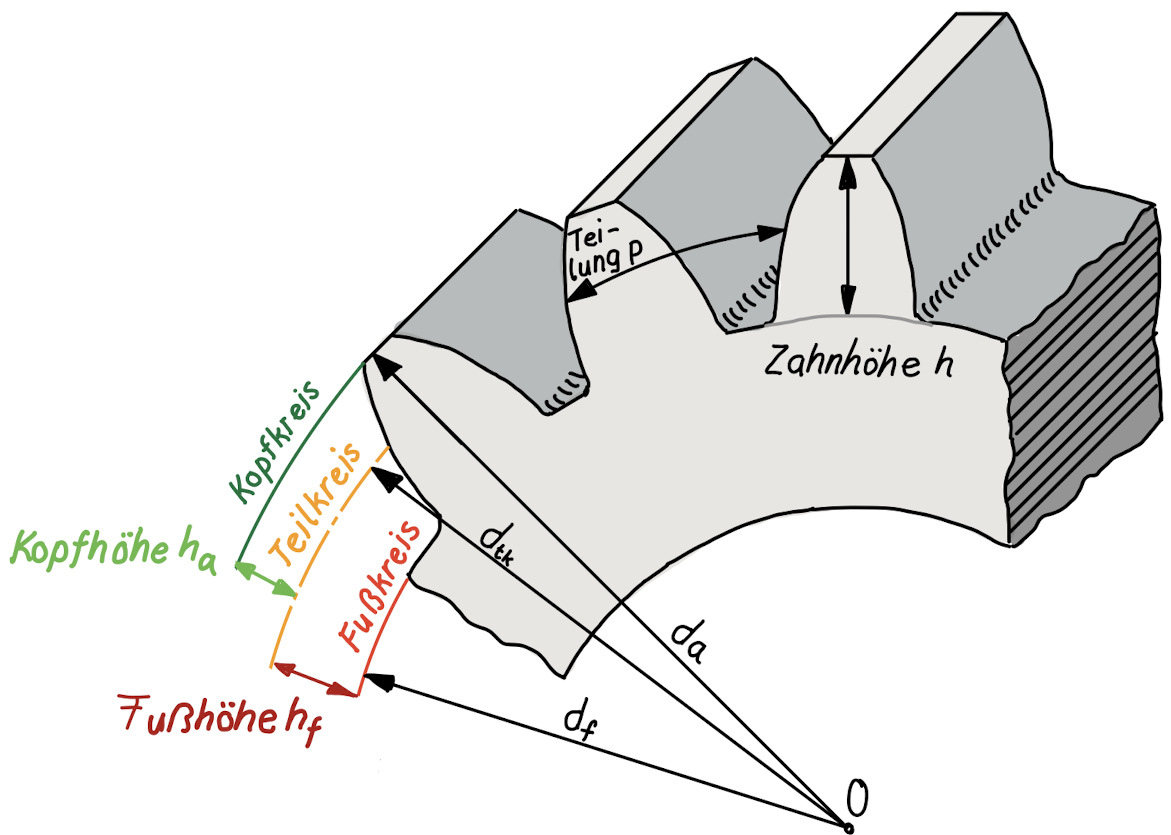
\includegraphics[width = 1.1\linewidth]{src/images/MAEIP_Zahnrad}
    \end{center}
\end{minipage}
\begin{minipage}{0.35\linewidth}
    \begin{center}
        \begin{scriptsize}
            \begin{align*}
                d_f &= \text{Fusskreis-} \varnothing
                \\d_{tk} &= \text{Teilkreis-} \varnothing
                \\d_a &= \text{Kopfkreis-} \varnothing
                \\ p&= \text{Teilung}
                \\ h_a &= \text{Zahnkopfhöhe} 
                \\ h_f &= \text{Fusshöhe}
                \\ h &= \text{Zahnhöhe}
             \end{align*}
        \end{scriptsize}    
    \end{center}
\end{minipage}

\begin{footnotesize}
    \begin{empheq}[box=\fbox]{align*}
        h = h_a + h_f \quad \mid \quad h_a = m \quad \mid \quad h_f = 1.1, ..., 1.3 \cdot m
    \end{empheq}
\end{footnotesize}

\subsubsection{Kräfte - geradverzahntes Zahnrad \hfill ME}
\vspace{-1mm}\begin{minipage}{0.4\linewidth}
    \begin{footnotesize}
        \begin{center}
            \mathbox{
                F_{t1} = F_{t2} = \frac{2M_1}{d_1}
            }
        \end{center}
    \end{footnotesize}
\end{minipage}
\begin{minipage}{0.58\linewidth}
    \begin{footnotesize}
        \begin{center}
            \mathbox{
                F_{r1} = F_{r2} = F_{t1} \cdot tan(\alpha)
            }
        \end{center}
    \end{footnotesize}
\end{minipage}

\subsubsection{Achsabstand $a$ \hfill ME}
\vspace{-1mm}
\mathbox{
    a = \frac{d_{tk1}}{2} + \frac{d_{tk2}}{2}
}
\vspace{0.1mm}